\documentclass[a4paper]{article}

% Language for grammar correction
\usepackage[american]{babel}
\usepackage[utf8]{inputenc}

% Type of the font
\usepackage[T1]{fontenc}
\usepackage[scaled]{helvet}
\renewcommand{\familydefault}{\sfdefault}

% Page side margin
\usepackage[margin=80pt]{geometry}

% Options for listings {enumerate, itemize, ...}
\usepackage{enumitem}
\setlist{nosep}

% recognize quotes as typed
\usepackage [autostyle]{csquotes}
\MakeOuterQuote{"}

% create code blocks with \begin{lstlisting}
\usepackage{listings}

% Hyperlinks without coloring
\usepackage[hidelinks]{hyperref}
\hypersetup{colorlinks=false}

% Used to insert Graphics
\usepackage{graphicx}

% Header and Footer configuration
\usepackage{fancyhdr}
\pagestyle{fancy}
\fancyhead{}
\fancyfoot{}

\rhead{I.BA\_AIOT.F1901}
\lhead{CasaGrama - Telegram Smart Home Bot}
\rfoot{Page \thepage}

% Lorem Ipsum through \lipsum[i]
\usepackage{lipsum}

\title{\textbf{CasaGrama - The Telegram Smart Home Bot}}
\author{Raphael Heer, Maurin Donat Thalmann\\
	HSLU, Informatik Department, Switzerland\\
	\emph{raphael.heer@hslu.ch, maurindonat.thalmann@stud.hslu.ch}}

\begin{document}
	
	\pagenumbering{gobble}
	\maketitle
	\newpage
	\pagenumbering{arabic}
	\tableofcontents
	\newpage
	
	\section{Abstract}
	
	The Internet of Things plays a huge role in the market for Smart Home devices. 
	Nowadays and in the future, people want their homes to behave as intelligent as possible, whenever and wherever they are. 
	But while it's an expensive task to fully automate your home, there's smaller and cheaper solutions to partially make your house smarter, so everyone should be able to "smart up" his house. \\
	The task of this paper is to develop a Telegram Bot, running on a dedicated server or cloud solution, which is able to control a number of IoT Smart Home devices. 
	Through the Telegram messenger application, one should be able to add, configure and control a handful of IoT devices. 
	So, for example, an LED or door lock can be (de-)activated or data sent from a sensor can be requested through the bot interface inside of the Telegram application. 
	Users should also be able to subscribe to specific devices, so the bot can notify them on a specified event.
	
	\paragraph{Telegram} 
	Telegram is a cloud-based instant messaging service, available on a wide range of platforms as Android, iOS, Windows, etc. 
	Besides communication between real-life persons, it supports the ability to communicate with Telegram bots. 
	These are running on dedicated servers and usually offer a range of commands to perform certain tasks within or outside of the Telegram application.
	
	\begin{figure}[htb!]
		\centering
		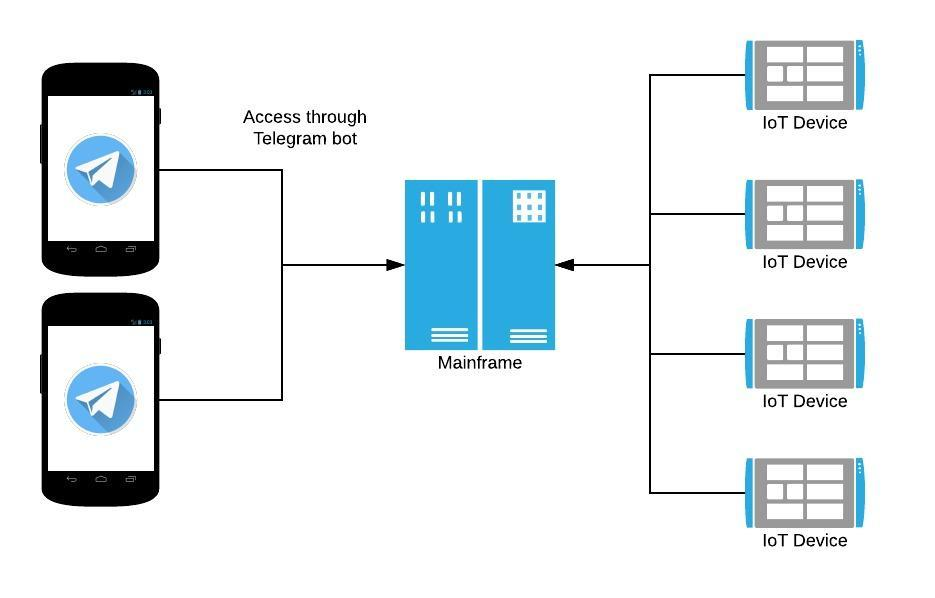
\includegraphics[width=.6\textwidth]{img/project_model.jpeg}
		\caption{Project Infrastructure Model}
	\end{figure}
	
	\section{Introduction}
	
	During this project, two main targets should be fulfilled for an ideal user experience.\\
	First target is to think of an intuitive way in which the user interacts with the bot. 
	How do the commands of the bot need to be set up, so that the user easily understands how he's able to control or read a certain device. 
	The second target is the functional range of the bot itself, which functions need to be covered and which ones can be marked as optional. 
	So in the following, the bot should be able to:
	\vspace{1em}
	\begin{itemize}
		\item Select a certain device from the range of connected devices
		\item Notify the user about certain device's events
		\item Perform a task on the selected device
			\begin{itemize}
				\item Read data from a device
				\item Change the state of a device (ON/OFF)
				\item Change the values of a device
			\end{itemize}
		\item Add / remove devices from the bot interface \textit{(optional)}
	\end{itemize}
\vspace{1em}
	We consider the project successful if we're able to access different types of devices or sensors through the bot interface. 
	The bot itself runs on an Azure cloud instance or at least uses their services. 
	The first version does not need to be capable of adding or removing other devices than the ones used during this project.
	
	\section{Related Work / Research}
	
	Throughout our research, we sought projects that would help us in the development of our Telegram bot and IoT devices we would want to be able to connect to. 
	Although we found several projects, most of them were in a foreign language we don't understand or just slightly helpful. 
	For example, there are several smaller DIY projects on the internet, for example:
	
	\begin{center}
		\textbf{How to Set Up Home Automation Through the Telegram Messenger App}\\
		\textit{\href{https://blog.hackster.io/how-to-set-up-home-automation-through-the-telegram-messenger-app-8551d6f493a1}
			{https://blog.hackster.io/how-to-set-up-home-automation-through-the-telegram-messenger-app-8551d6f493a1}}\\
		\textbf{Home Automation With Telegram Bot}\\
		\textit{\href{http://www.lucadentella.it/en/2015/10/13/automazione-con-bot-telegram/}
			{http://www.lucadentella.it/en/2015/10/13/automazione-con-bot-telegram/}}\\
		\textbf{Telegram bot for chatting with arduino - Smart Home}\\
		\textit{\href{https://www.youtube.com/watch?v=UrwlOUQ1JMc}{https://www.youtube.com/watch?v=UrwlOUQ1JMc}}
	\end{center}
	\noindent
	These are simple examples of Telegram bots to control a light chain or to read data from sensors. 
	Unfortunately, they aren't very well documented and are very basic in functionality. 
	But only the fact to see something working, similiar to what we want to achieve, was kind of impressive. 
	The last link leads to a YouTube video of a Telegram bot, receiving input from a button and controlling a LED light, which is apparently connected through Azure (as far as the description tells us). 
	Sadly this is even less documented that the other examples, therefore it wasn't of help for our project as well.\\
	For the development of the Telegram bot, we've consulted the official Telegram bot API and several tutorials to create first Telegram bots. 
	While working through some of these tutorials, we've discovered a git repository for an (apparently) well-known wrapper for the Telegram bot API:
	\begin{center}
		\textbf{GitHub : python-telegram-bot}\\
		\textit{\href{https://github.com/python-telegram-bot/python-telegram-bot}{https://github.com/python-telegram-bot/python-telegram-bot}}
	\end{center}
	The \textit{python-telegram-bot} is a package that wraps the Telegram bot API into easily understandable classes. 
	It has a huge community, a well-documented API and a wiki with tutorials, code snippets and also bot examples, created by other users. 
	We've also found other wrappers like this, but in the end we decided to use this one for its simple usage and big community.\\
	The documentation for the Azure Python SDK contains a lot of tutorials, well-documented APIs as well as examples of real-life use cases, from which we were able to derivate several code snippets into our own project.
	
	\newpage
	\section{System Design and Implementation}
	As cloud infrastructure platform, we chose Microsoft Azure services, for which we were granted access by the HSLU.
	The main application of the Telegram Bot is written in Python.
	The IoT devices are connected to the Azure Cloud through WLAN.
	
		\subsection{System Overview}
		
	
		A diagram of the whole system overview can be found on the next page.\\
		The system of the prototype is divided into multiple sections, which will be described in the following:\\
		
		\begin{itemize}[itemsep=1em]
			\item \textbf{User Side:} An end user is able to access the Telegram application on a device (smartphone, laptop etc.). 
			Through this application, he can start a conversation with our Telegram Bot to access its features.
			
			\item \textbf{Telegram Servers:} Every action performed in the Telegram application is processed by the Telegram servers.
			So every request by a user to our Bot is first received by the Telegram servers and processed through to our Bot application.
			
			\item \textbf{Telegram Bot}: This is the main entry point for user requests.
			It is a Python script running on a dedicated server or computer.
			The user invokes a command over Telegram which is finally received by the Telegram bot.
			In here, the request is forwarded to a subclass of our Bot, which then communicates with the Azure Cloud.
			This defines the Telegram Bot as the main node between the Telegram servers and the Azure Cloud.
			There is and must only run one Telegram Bot instance at a time.
			For this reason, the Python script must include a unique bot token, generated by the BotFather Bot on the Telegram servers.
			
			\item \textbf{Microsoft Azure}:	In contrary to the other applications, Azure is less about programming and more about configuration.
			Therefore, the required services on the Azure Cloud must be configured for our exact needs.
			To be able to write data into the Cosmos DB, a Stream Analytics service must be running which listens to data sent by an IoT device in the IoT Hub.
			Every IoT device needs to be configured as such in an IoT Hub instance.
			
			\item \textbf{IoT Device Applications}: The last section are the IoT devices and their applications. 
			Their task is to interact with their distinct peripherals and communicate with the Azure Cloud, more precisely to send and receive data.
		\end{itemize}
	
		\newpage
	
		\begin{figure}[!htb]
			\centering
			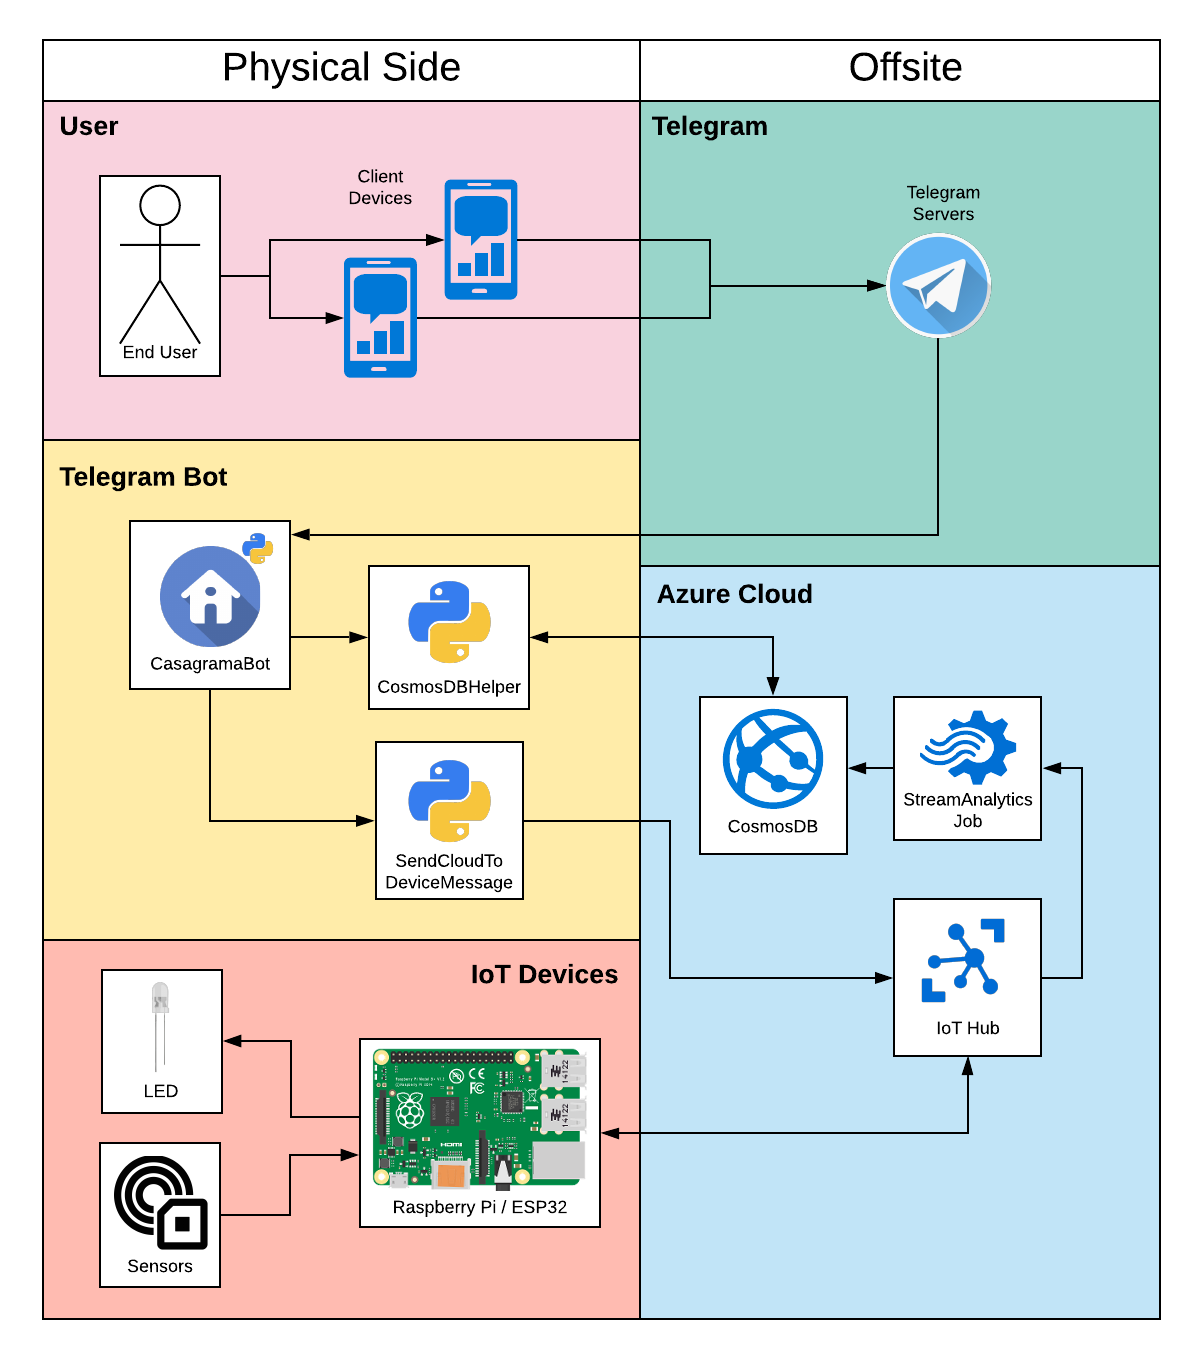
\includegraphics[width=\textwidth]{img/overview.png}
			\caption{Overview of the whole prototype system}
			\label{fig:systemoverview}
		\end{figure}
	
		\newpage
		
		\subsection{System Architecture}
		
			\subsubsection{Telegram Bot}
			
			The Telegram Bot is actually divided into a main application and two subclasses.
			Logging has been implemented in all of them to guarantee the right functionality.\\
			
			The \textbf{CasaGramaBot} serves as the main application of the Bot.
			It contains the bot token to access the Telegram Bot API and the necessary attributes to access the Cosmos DB.
			If an user enters a command on his client, it will be handled and forwarded to the appropriate function.\\
			
			The \textbf{CosmosDBHelper} is called in the main application to access the latest entry of the Cosmos DB we used during this project.
			It receives the URL and access key it needs to access the Cosmos DB from the main application.
			It simply reads the database and the latest entry of its table and is able to return the required attributes.\\
			
			The \textbf{SendCloudToDeviceMessage} is called in the main application as well.
			It contains the connection string to the IoT Hub itself and the device ID it wants to communicate with.
			Its sole purpose for this project is to send a message to the Raspberry Pi, through which the Raspberry Pi knows what to do with the LED.
			When it is called in the main application, it receives the state that the LED should be in as the \texttt{command} parameter.
			
			
			\begin{figure}[!htb]
				\centering
				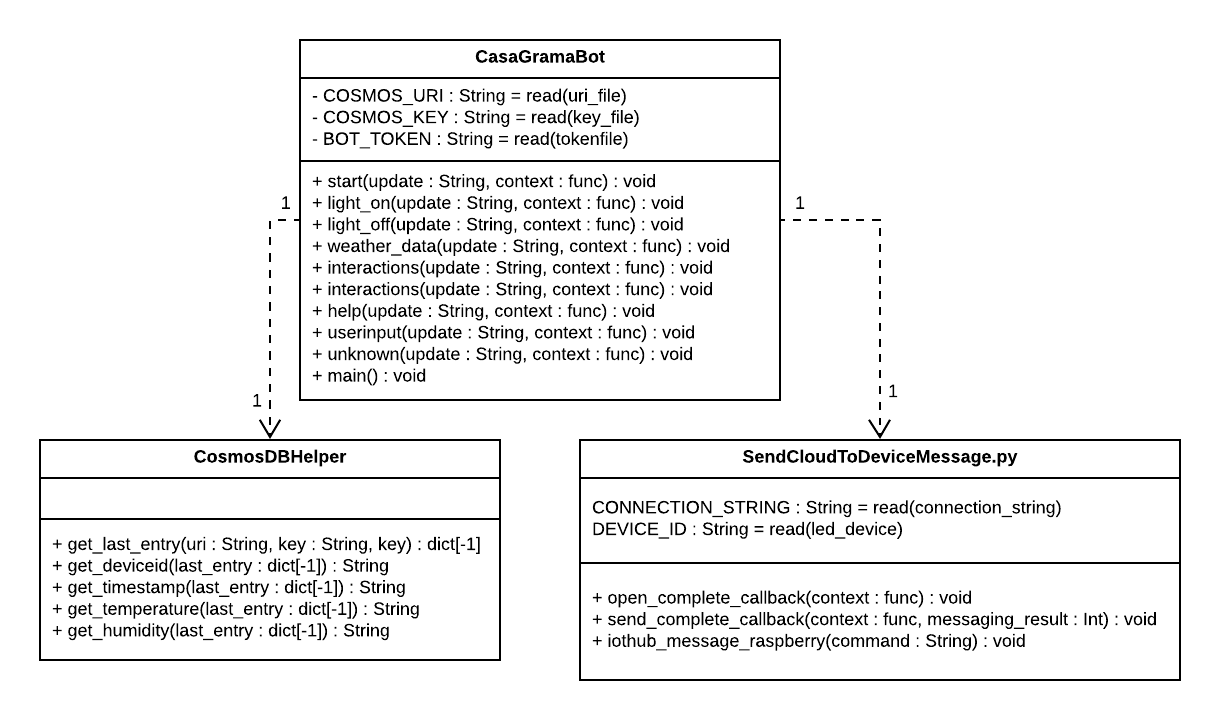
\includegraphics[width=\textwidth]{img/bot_classdiagram.png}
				\caption{Class diagram of the Telegram Bot application}
				\label{fig:botclassdiagram}
			\end{figure}
		
			\newpage
		
			\subsubsection{IoT Devices}
			Theoretically, there could be a large amount of IoT Devices which are running with different applications and communicating with the cloud.
			This is what the Azure IoT Hub was made for.
			However, this would require some prior knowledge about the different technologies on the devices and in the cloud.
			Due to this reason, the project uses only two types of applications which are implemented on the Raspberry Pi.
			\\
			\\
			The applications were divided into two categories.
			Both categories are implemented to be extendable with other use cases.
			They are described in the following paragraphs:

			\paragraph{Send Data to the Azure IoT Hub with a BME280}
			
			The goal of the first use case is to send data continuously to the Azure IoT Hub.
			In the cloud, the data will be processed with Stream Analytics and afterwards saved to Cosmos DB.
			The data flow in this application is just in one direction from the Raspberry Pi to the cloud.
			In this project, the BME280 sensor was used.
			It measures the temperature, the humidity and the air pressure.
			For other projects, the BME280 sensor can be exchanged with any other sensor that collects data from its environment.
			\\
			\\
			Following class diagram shows the class structure of the application:
			
			\begin{figure}[!htb]
				\centering
				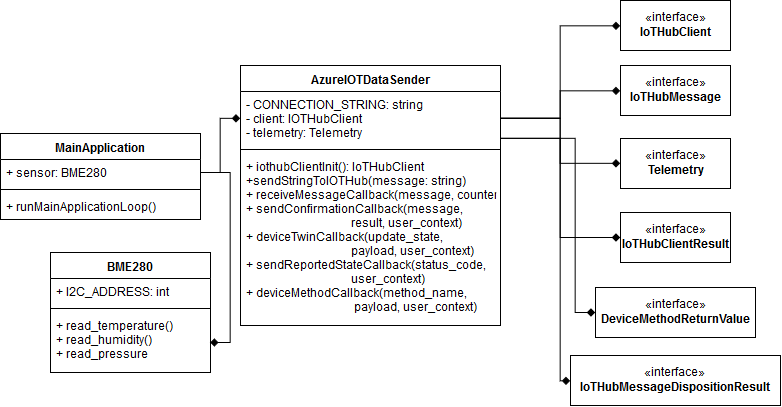
\includegraphics[width=\textwidth]{img/raspberry_bme280_application.png}
				\caption{Class diagram for the weather data application}
				\label{fig:raspibme280class}
			\end{figure}
			
			\newpage
			
			\paragraph{Listen to commands from the Azure IoT Hub and turn the lights on and off}

			The goal of the second application is to receive commands from the cloud and perform a pre defined action.
			The action is issued from the user over the Telegram Bot.
			The telegram bot sends a message over the Azure IoT Hub to the device.
			The device, which is listening to the Azure IoT Hub, receives the message.
			In this project, an LED can be turned off and on by over the Telegram Bot.
			For other projects, it could be possible to open the window or inform the user, that the clothes in the washing machine are ready to be taken out.
			\\
			\\
			Following class diagram shows the class structure of the application:
			\begin{figure}[!htb]
				\centering
				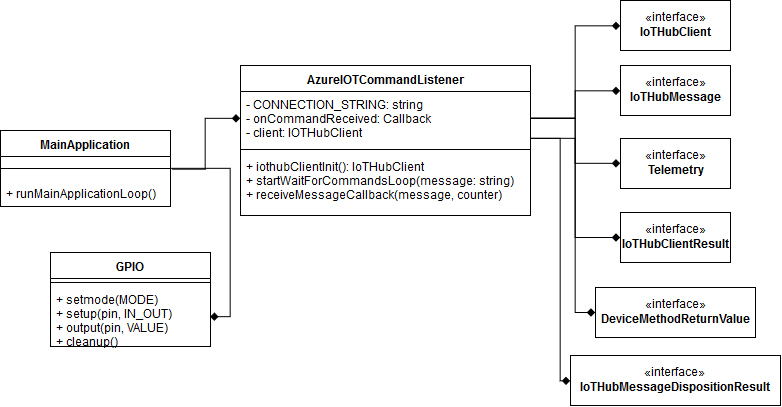
\includegraphics[width=\textwidth]{img/raspberry_led_application.png}
				\caption{Class diagram for the LED application}
				\label{fig:raspiledclass}
			\end{figure}
			
		
		\newpage
		\subsection{Software Architecture Layers \& Modules}
		
			\subsubsection{Telegram Bot}
					
				\paragraph{CasaGramaBot}
							
				\def\arraystretch{1.25}
				\begin{table} [h!]
				\centering
					\begin{tabular} [h!] { | p{5.5cm} | p{9cm} | }
						\hline
						\multicolumn{ 2 }{ | c | }{\textbf{Telegram Bot - CasaGramaBot.py}} \\
						\hline\hline
						\textbf{Interface} & \textbf{Description} \\
						\hline
						\multicolumn{ 2 }{ | c | }{\textbf{Provides}} \\
						\hline
						
						\texttt{start(update, context)} & Returns a start message, invoked by the \texttt{\textbackslash start} command. \\
						\texttt{light\_on(update, context)} & Turns the light on for an IoT device, invoked by the \texttt{\textbackslash light\_on} command. \\
						\texttt{light\_off(update, context)} & Turns the light off for an IoT device, invoked by the \texttt{\textbackslash light\_off} command. \\
						\texttt{weather\_data(update, context)} & Returns the most recent weather data from an IoT device, invoked by the \texttt{\textbackslash weather\_data} command. \\
						\texttt{interactions(update, context)} & Returns a custom keyboard to select different interactions, invoked by the \texttt{\textbackslash interactions} command. \\
						\texttt{help(update, context)} & Returns a help message, invoked by the \texttt{\textbackslash help} command.  \\
						\texttt{userinput(update, context)} & Logs text messages sent by a client. \\
						\texttt{unknown(update, context)} & Returns error message for unknown commands, invoked by any unknown command. \\
						\texttt{main()} & Starts the Telegram Updater and binds all commands to handlers. \\
						
						\hline\hline
						\textbf{Interface} & \textbf{Description} \\
						\hline
						\multicolumn{ 2 }{ | c | }{\textbf{Uses}} \\
						\hline
						
						\texttt{telegram.ext.Updater()} & Enables retrieving of updates with the Telegram Bot API, needs to be given a Bot token. \\
						\qquad\texttt{*.startPolling()} & Starts communication and starts listening for actions. \\ 
						\hline
						\texttt{telegram.ext.CommandHandler()} & Handles commands received by the bot from a client, needs to be given a command name and the action to be fulfilled. \\
						\texttt{telegram.ext.MessageHandler()} & Handles messages received by the bot, needs to be given a message filter and the action to be fulfilled. \\
						\texttt{telegram.ext.Filters()} & Filter incoming messages by content or type (e.g. messages, commands) \\ 
						\hline
						\texttt{telegram} & \\
						\qquad\texttt{*.KeyboardButton()} & Defines a button for a custom keyboard.  \\
						\qquad\texttt{*.ReplyKeyboardMarkup()} & Enables a custom keyboard in a Telegram client. \\ 
						\hline
						\texttt{logging.getLogger()} & Activates Logging for this script. \\
						\texttt{logging.basicConfig()} & Configures logging aspects, like formatting, log level etc. \\
						\texttt{logging.FileHandler()} & Enables logging to a file in a given directory. \\
						\texttt{logging.StreamHandler()} & Enables logging to the console. \\	
						\hline				
					\end{tabular}
					\caption{Interfaces used from Libraries and Methods used in CasaGramaBot}
					\label{tab:bot_int}
				\end{table}
		
				The \texttt{CasaGramaBot.py} is the main application which needs to be executed in order to run the Telegram bot. 
				It uses the interfaces from \textit{python-telegram-bot} to access the Telegram Bot API in turn to communicate with a Telegram client.
		
				\newpage
		
				\paragraph{CosmosDBHelper}
			
				\def\arraystretch{1.3}
				\begin{table} [h!]
					\centering
					\begin{tabular} [h!] { | p{5.8cm} | p{8.7cm} | }
						\hline
						\multicolumn{ 2 }{ | c | }{\textbf{Telegram Bot - CosmosDBHelper.py}} \\
						\hline\hline
						\textbf{Interface} & \textbf{Description} \\
						\hline
						\multicolumn{ 2 }{ | c | }{\textbf{Provides}} \\
						\hline
						%TODO
						\texttt{get\_last\_entry(uri, key)} & Gets the latest (most recent) database entry, needs to be given the database's URL and the access key. \\
						\texttt{get\_temperature(last\_entry)} & Get the temperature value from the latest entry, needs to be given the latest entry. \\
						\texttt{get\_humidity(last\_entry)} & Get the humidity value from the latest entry, needs to be given the latest entry. \\
						
						\hline\hline
						\textbf{Interface} & \textbf{Description} \\
						\hline
						\multicolumn{ 2 }{ | c | }{\textbf{Uses}} \\
						\hline
						
						\texttt{document\_client.DocumentClient()} & Creates a connection to a database, needs to be given the database URL and the access key. \\
						\quad\texttt{.QueryDatabases()} & Reads databases from a database connection, needs to be given a query. \\
						\quad\texttt{.QueryCollections()} & Reads tables or collections from a database, needs to be given a query. \\
						\quad\texttt{.ReadDocuments()} & Reads documents in a table or collection, needs to be given a query. \\ 
						\hline
						\texttt{logging.getLogger()} & Activates Logging for this script. \\
						\texttt{logging.basicConfig()} & Configures logging aspects, like formatting, log level etc. \\
						\texttt{logging.FileHandler()} & Enables logging to a file in a given directory. \\
						\texttt{logging.StreamHandler()} & Enables logging to the console. \\	
						\hline
					\end{tabular}
					\caption{Interfaces used from Libraries and Methods used in CosmosDBHelper}
					\label{tab:dbhelper_int}
				\end{table}
		
				The \texttt{CosmosDBHelper.py} serves as a connection helper to our Azure Cosmos DB to receive the latest weather data. 
				It uses the interface \textit{document\_client} from the Python package \textit{pydocumentdb}, which allows to query entries from a database. \\
				It is used by the main application to 
			
				\newpage
				
				\paragraph{SendCloudToDeviceMessage}
			
				\def\arraystretch{1.3}
				\begin{table} [h!]
					\centering
					\begin{tabular} [h!] { | p{5.9cm} | p{8.6cm} | }
						\hline
						\multicolumn{ 2 }{ | c | }{\textbf{Telegram Bot - SendCloudToDeviceMessage.py}} \\
						\hline\hline
						\textbf{Interface} & \textbf{Description} \\
						\hline
						\multicolumn{ 2 }{ | c | }{\textbf{Provides}} \\
						\hline
						%TODO
						\texttt{open\_complete\_callback(context)} & Logs the callback for opened communication \\
						\texttt{close\_complete\_callback(context)} & Logs the callback for closed communication, needs to be given messaging result. \\
						\texttt{iothub\_message\_raspberry(command)} & Sends a message to the predefined device in the IoT Hub, needs to be given a message to be sent. \\
						
						\hline\hline
						\textbf{Interface} & \textbf{Description} \\
						\hline
						\multicolumn{ 2 }{ | c | }{\textbf{Uses}} \\
						\hline
						%TODO
						\texttt{iothub\_service\_client} & Package for the IoT Hub Message sender / service \\
						\quad\texttt{.IoTHubMessaging()} & Enables communication with an IoT Hub instance, needs to be given the connection string to the IoT Hub.\\
						\qquad\texttt{.open()} & Opens communication with the IoT Hub, needs to be given a callback and context. \\
						\qquad\texttt{.sendasync()} & Sends a cloud-to-device message in the IoT Hub, needs to be given a device name, message, callback and message index. \\
						\qquad\texttt{.close()} & Ends communication with the IoT Hub. \\
						\quad\texttt{.IoTHubMessage()} & Object which can be delivered to a target device in the IoT Hub, needs to be given message content. \\
						\quad\texttt{.IoTHubError()} & An exception which can be thrown when there are problems with the connection to the IoT Hub \\ 
						\hline
						\texttt{logging.getLogger()} & Activates Logging for this script. \\
						\texttt{logging.basicConfig()} & Configures logging aspects, like formatting, log level etc. \\
						\texttt{logging.FileHandler()} & Enables logging to a file in a given directory. \\
						\texttt{logging.StreamHandler()} & Enables logging to the console. \\	
						\hline
					\end{tabular}
					\caption{Interfaces used from Libraries and Methods used in SendCloudToDeviceMessage}
					\label{tab:dbhelper_int}
				\end{table}
		
				The \texttt{SendCloudToDeviceMessage.py} makes Cloud-to-device messaging possible for our Bot. It utilizes the Python package \textit{azure-iothub-service-client}, which serves as a handler for cloud-to-device messages.
		
		\newpage
		
			\subsubsection{IoT Devices}
			There are two different kinds of applications for the IoT Devices.
			The first type continuously sends data to the Azure IoT Hub.
			It does not receive any input from the IoT Hub except for the confirmation messages.
			The second one listens to the Azure IoT Hub and waits for a command to execute some functionality like turning the lights on or off.\\
			\\
			For this reasons, there are two types of wrapper classes, which wraps exactly this functionality.
			They are called \texttt{AzureIOTDataSender} and \texttt{AzureIOTCommandListener}.
			The code for this classes is derived from an example application to communicate with Azure IoT Hub.			
			Which methods they provide and which methods they use is described in the following two tables.
			
				\paragraph{AzureIOTDataSender}
				
				\def\arraystretch{1.2}
				\begin{table} [h!]
					\centering
					\begin{tabular} [h!] { | p{5.9cm} | p{8.6cm} | }
						\hline
						\multicolumn{ 2 }{ | c | }{\textbf{Raspberry Pi - AzureIOTDataSender}} \\
						\hline\hline
						\textbf{Interface} & \textbf{Description} \\
						\hline
						\multicolumn{ 2 }{ | c | }{\textbf{Provides}} \\
						\hline
						
						\texttt{\_\_init\_\_(connectionString)} & Constructor for the class AzureIOTHubDataSender \\
						\texttt{iothubClientInit()} & This method is used to create an instance of the class IoTHubClient. This object is used to send data to the IoT Hub. \\
						\texttt{sendStringToIOTHub(messageString)} & Sends a string to the Azure IOT Hub. \\
						\texttt{receiveMessageCallback(message, counter)} & Callback function. Is called if the IoT Hub sends a message to the device. \\
						
						\texttt{sendConfirmationCallback(} \quad \texttt{message, result, user\_context)} & Callback function. Is called after the IoT Hub sends a confirmation that the message has been received. \\
						\texttt{deviceTwinCallback(update\_state, payload, user\_context)} & Callback function. Called for Digital Twins functionallity \\
						\texttt{sendReportedStateCallback(} \quad \texttt{status\_code, user\_context)} & Callback function. Is called, if the reported state has been received by the IoT Hub \\
						\texttt{deviceMethodCallback(method\_name, payload, user\_context)} & Callback function. Is called if the device receives a message \\
												
						\hline\hline
						\textbf{Interface} & \textbf{Description} \\
						\hline
						\multicolumn{ 2 }{ | c | }{\textbf{Uses}} \\
						\hline
						
						\texttt{IoTHubClient} &  \\
						\quad\texttt{.send\_event\_async(message, confirmationCallback, messageCount)} & Send asynchronous message to the IoT Hub \\
						\quad\texttt{.send\_reported\_state(} \quad \texttt{reported\_state, str\_length, reportedStateCallback, context)} & Report IoTHubClient state to Azure \\
						\texttt{Telemetry} & \\
						\quad\texttt{.send\_telemetry\_data( \quad IoTHubName, str\_length, event\_success, message)} & Send telemetry data to Azure \\
						
						
						\hline				
					\end{tabular}
					\caption{Interfaces used from the main application to communicate with the Azure IoT Hub}
					\label{tab:send_to_iot}
				\end{table}
				
				The \texttt{AzureIOTDataSender.py} is the part of the application, which communicates with the Azure IoT Hub. It is wrapper for all the Azure features like Telemetry and IoTHubClient.
		
				\newpage
		
				\paragraph{AzureIOTCommandListener}
				
				\def\arraystretch{1.2}
				\begin{table} [h!]
					\centering
					\begin{tabular} [h!] { | p{5.9cm} | p{8.6cm} | }
						\hline
						\multicolumn{ 2 }{ | c | }{\textbf{Raspberry Pi - AzureIOTCommandListener}} \\
						\hline\hline
						\textbf{Interface} & \textbf{Description} \\
						\hline
						\multicolumn{ 2 }{ | c | }{\textbf{Provides}} \\
						\hline
						
						\texttt{\_\_init\_\_(connectionString)} & Constructor for the class AzureIOTHubCommandListener \\
						
						\texttt{iothubClientInit()} & This method is used to create an instance of the class IoTHubClient. This object is used to send data to the IoT Hub. \\
						
						\texttt{startWaitForCommandsLop( \quad onCommandReceivedCallback)} & Starts the loop to wait for commands. \\
						
						\texttt{receiveMessageCallback(message, counter)} & Callback function. Is called if the IoT Hub sends a message to the device. \\

						\hline\hline
						\textbf{Interface} & \textbf{Description} \\
						\hline
						\multicolumn{ 2 }{ | c | }{\textbf{Uses}} \\
						\hline
						
						\texttt{IoTHubClient} &  \\
						\quad\texttt{.set\_message\_callback( \quad callbackFunction, RECEIVE\_CONTEXT)} & Sets the callback function which is called if the IoT Hub sends a message \\
						
						
						\hline				
					\end{tabular}
					\caption{Interfaces used from the main application to receive messages from the Azure IoT Hub}
					\label{tab:listen_to_iot}
				\end{table}
				
				The \texttt{AzureIOTCommandListener.py} is the part of the application, which communicates with the Azure IoT Hub. It is wrapper for all the Azure features like IoTHubClient. It receives the IoTHubMessage, gets the actual message from it and calls a given callback.
		
		\newpage
		
		\subsection{System Implementation / Functional Software Architecture}
		
			\subsubsection{Telegram Bot}
			
			For the Telegram bot to work, some requirements have to be met before running it.\\
			
			\begin{itemize}
				\item \textbf{Required packages}\\
				There are a couple of packages, as mentioned in previous chapters, which need to be installed for the Bot to work.
				We created a requirements file with the console application \texttt{pipreqs}, which outputs a requirements text file.
				Through \texttt{pip} (Python package manager) the requirements file can be handed over as a parameter and \texttt{pip} will install the required packages by itself.
				The required packages are:
					\begin{itemize}
						\item \texttt{python-telegram-bot}
						
						\item \texttt{pydocumentdb}
						
						\item \texttt{telegram}
						
						\item \texttt{azure-iothub-service-client}\\
						\textit{(On Windows, this package can easily be installed through \texttt{pip}.
						On Mac/Linux, you need to clone the Azure IoT Hub C SDK from Github and compile it yourself.
						A guide on how to do this can be found on the Azure IoT Hub Python SDK repository on Github)}\\
					\end{itemize}
				
				\item \textbf{Required values}\\
				There are some values which need to be created so the Bot knows how he is able to communicate with Azure.
				The required values have been outsourced from the script into the folder \texttt{properties} and are read during runtime.
				Following are the names of the files and what they should contain:\\
					\begin{itemize}
						\item \texttt{TOKEN.txt}\\
						This file contains the Telegram bot token for your Bot.
						As mentioned, it needs to be generated by starting a chat with the \textit{@BotFather} on Telegram and creating a new bot instance.\\
						It is accessed in the CasaGramaBot.py file.
						
						\item \texttt{COSMOSDB\_READKEY.txt}\\
						This file contains the first access key to your Cosmos DB, which can be read directly from the Cosmos DB instance in Azure.\\
						It is accessed in the CasaGramaBot.py file.
						
						\item \texttt{COSMOSDB\_URI.txt}\\
						This file contains the URL which allows a connection to your Cosmos DB. It can also be retrieved directly from your Cosmos DB instance.\\
						It is accessed in the CasaGramaBot.py file.
						
						\item \texttt{CONNECT\_STRING.txt}\\
						This file contains the connection string of the IoT Hub containing the device whose LED should be controlled.
						It can be accessed by navigating to the access control of the IoT Hub and getting the connection string of a IoT Hub owner.\\
						It is accessed in the SendCloudToDeviceMessage.py file
						
						\item \texttt{LED\_DEVICE.txt}\\
						This file contains the name of the device whose LED should be controlled.
						The device name can easily be found in the IoT Hub which contains it.\\
						It is accessed in the SendCloudToDeviceMessage.py file.\\
						
					\end{itemize}
				
				\item \textbf{Running the bot}\\
				If all the requirements above are met, simply navigate to the \texttt{CasaGramaBot} directory and run the script with Python 3 as followed:\\
				(The project was tested with Python 3.7, we cannot guarantee it works under Python 2.7 due to incompatibility issues)\\
				\\
				\texttt{python3 CasaGramaBot.py}
				
			\end{itemize}
			
			\newpage
			
			\subsubsection{IoT Devices}
			
			Following is described how the applications are implemented and how to set them up for running.
			
			\paragraph{BME280 application on the Raspberry Pi}
			
			\begin{itemize}
				\item \textbf{Required packages for the BME280 application on the Raspberry Pi}\\
				There are two packages which are needed in order to run this application. 
				The driver for the \texttt{BME280 sensor} can be installed over "\texttt{pip3 install adafruit-circuitpython-bme280}".
				The \texttt{azure-iothub-device-client} is not installable over \texttt{pip}.
				It needs to be pulled from the Github Repository of Microsoft and compiled by the user himself.
				Since the application only runs on the Raspberry Pi, the package is deployed with source code.
			
				\item \textbf{Wiring the Raspberry Pi with the BME 280}
				Wire the Raspberry Pi and the BME 280 Sensor like in the following picture:
				\\
				Here will be an image of the wiring
				\\
				\item \textbf{Required values}\\
				There are different values which can be set to configure the application.
				Some are required and some are optional with a default value.
				To change this values, open the \texttt{config.py} file in the \texttt{RASPBERRY\_PYTHON\_BME280} and set the values.
				\begin{itemize}
					\item \texttt{CONNECTION\_STRING}(\textbf{required}): Connection string for the device to connect to the Azure IoT Hub
					\item \texttt{SLEEP\_DELAY\_IN\_S}(optional): Time in seconds to wait between messages
					\item \texttt{I2C\_ADDRESS}(optional): Address of the \texttt{BME280 Sensor}
					\\
				\end{itemize}
				
				\item \textbf{Running the application}
				If all the requirements above are met, simply navigate to the \\ \texttt{RASPBERRY\_PYTHON\_BME280} directory and run the script with Python 3 as followed:
				\\
				\texttt{python3 BME280\_Application.py}
			\end{itemize}
		
			\begin{figure}[!htb]
				\centering
				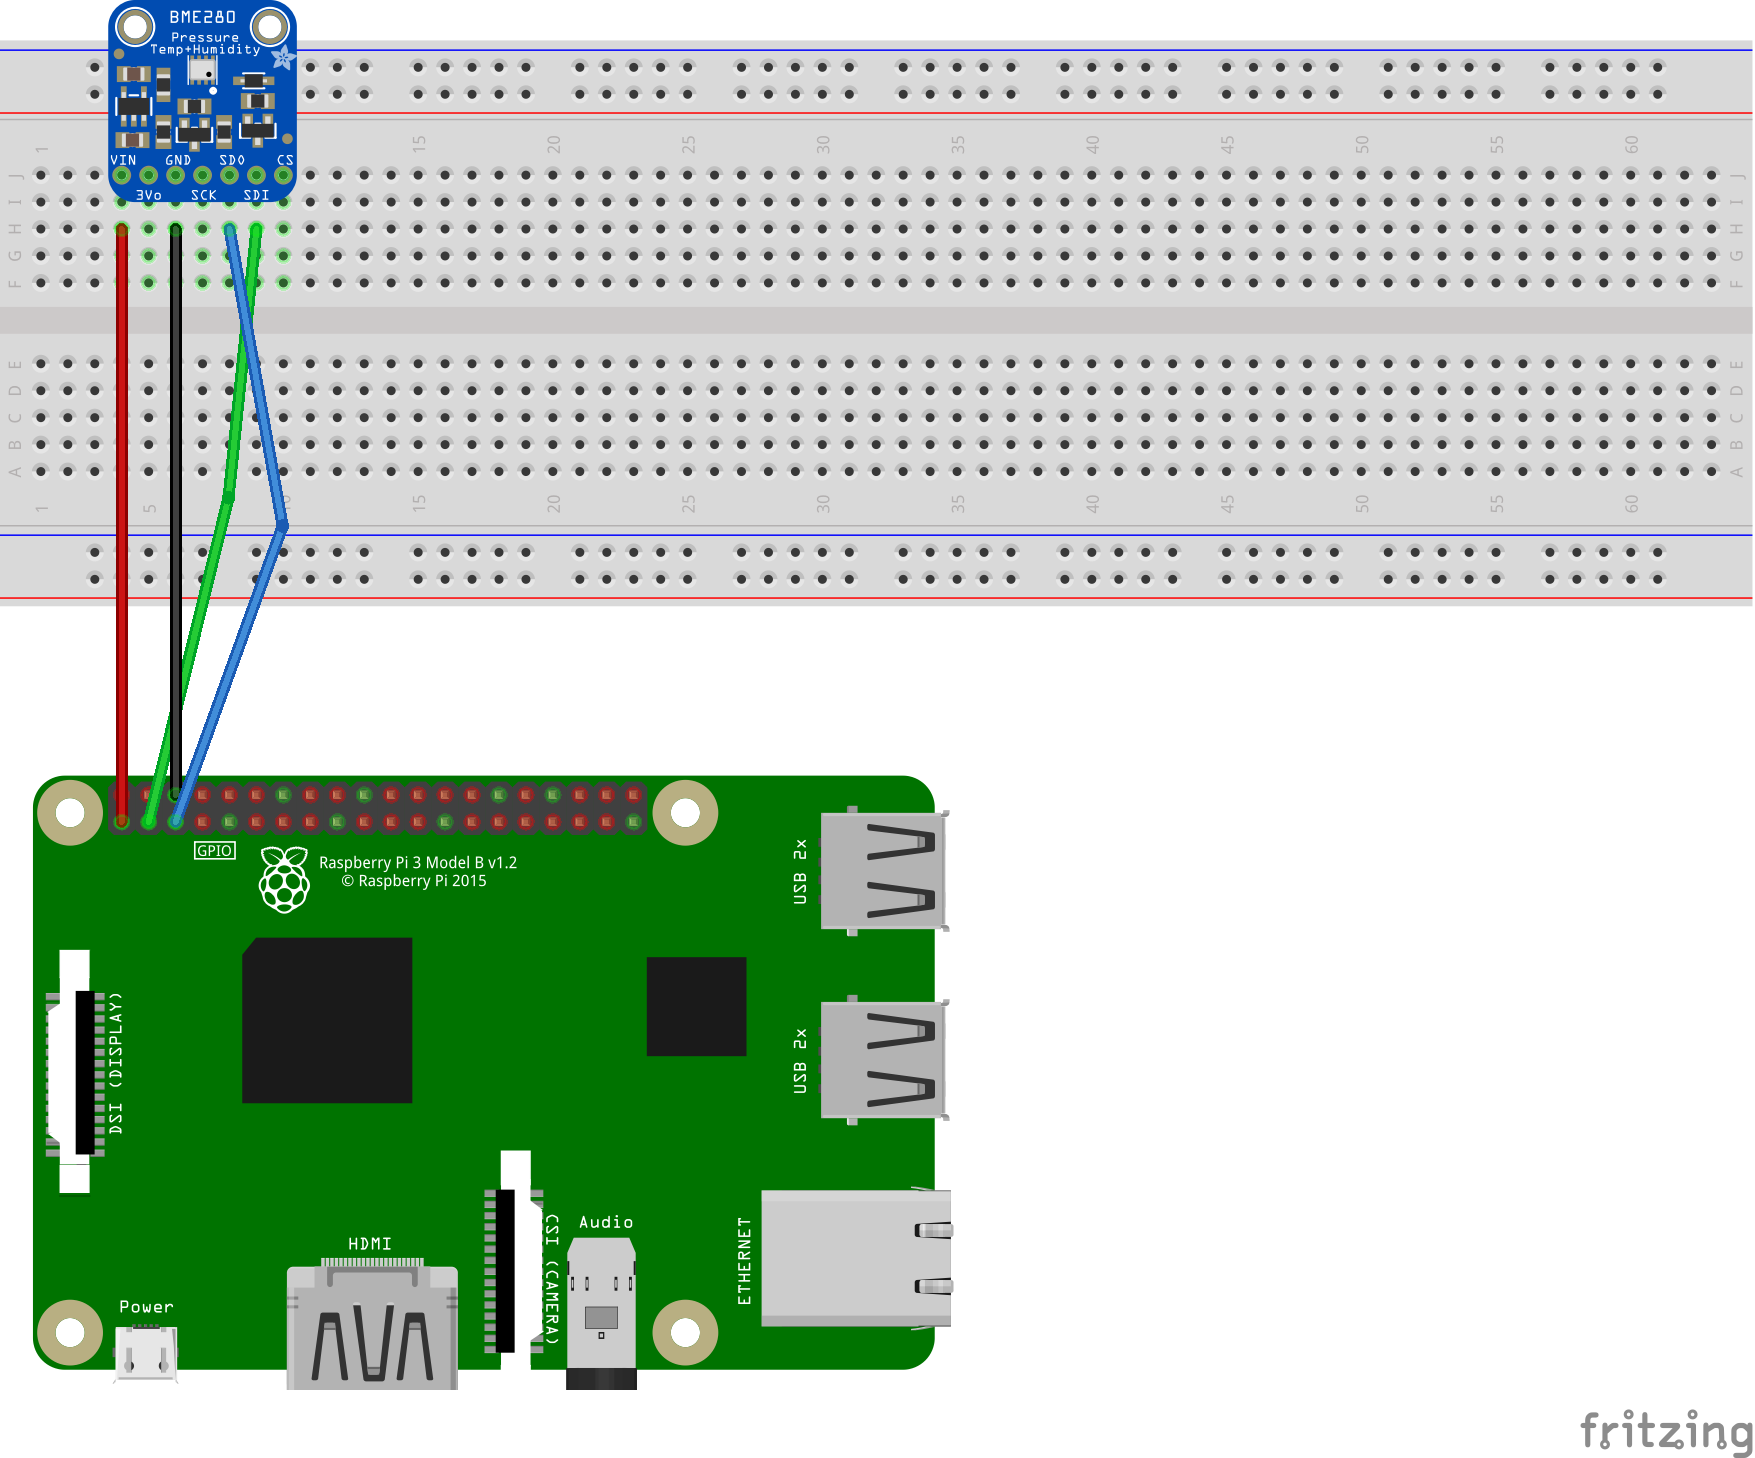
\includegraphics[width=.8\textwidth]{img/raspberry_bme280_wiring.png}
				\caption{Wiring diagram for the BME280}
				\label{fig:wiringbme280}
			\end{figure}
			
			\newpage
			
			\paragraph{LED application on the Raspberry Pi}
				
				\begin{itemize}
				\item \textbf{Required packages}\\
				There are two packages which are needed in order to run this application. 
				The first one is the library to handle the output over the GPIO.
				It can be installed with "\texttt{pip3 install RPi.GPIO}".
				The \texttt{azure-iothub-device-client} is not installable over \texttt{pip}.
				It needs to be pulled from the Github Repository of Microsoft and compiled by the user himself.
				Since the application only runs on the Raspberry Pi, the package is deployed with source code.
				\\
				\item \textbf{Wiring the Raspberry Pi with the LED}
				\\
				Wire the Raspberry Pi and the LED like in the following picture:
				\\
				\item \textbf{Required values}\\
				There are different values which can be set to configure the application.
				Some are required and some are optional with a default value.
				To change this values, open the \texttt{config.py} file in the \texttt{RASPBERRY\_PYTHON\_LED} and set the values.
				\begin{itemize}
					\item \texttt{CONNECTION\_STRING}(\textbf{required}): Connection string for the device to connect to the Azure IoT Hub
					\item \texttt{GPIO\_PIN}(optional): Address of the \texttt{BME280 Sensor}
					\\
				\end{itemize}
				
				
				\item \textbf{Running the application}
				If all the requirements above are met, simply navigate to the \\ \texttt{RASPBERRY\_PYTHON\_LED} directory and run the script with Python 3 as followed:
				\\
				\texttt{python3 LED\_Application.py}
				
			\end{itemize}
			
			\begin{figure}[!htb]
				\centering
				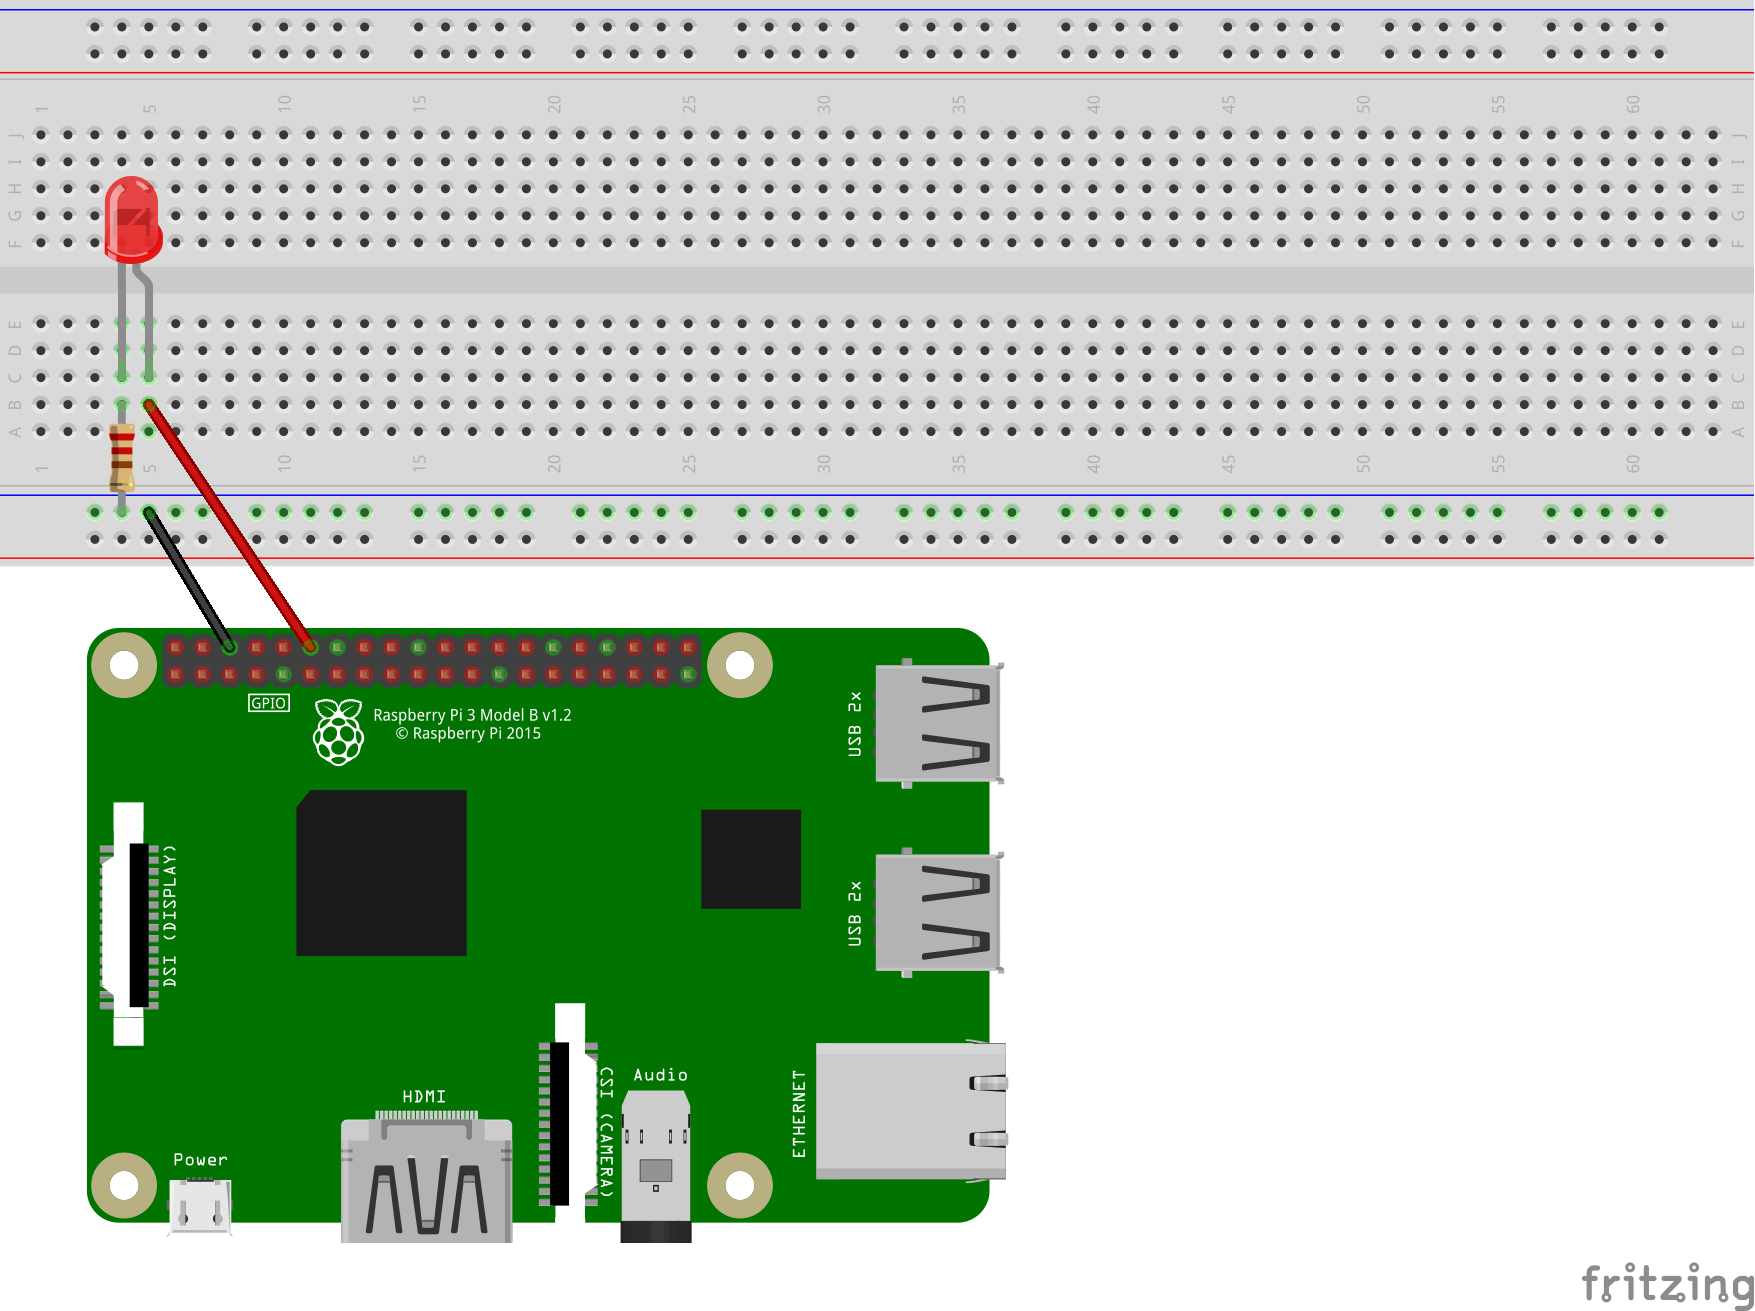
\includegraphics[width=.8\textwidth]{img/raspberry_led_wiring.png}
				\caption{Wiring diagram for the Raspberry Pi with LED}
				\label{fig:wiringled}
			\end{figure}
			
			
		
	\newpage
	\section{Evaluation / Experiments / Results / Discussion}
	
		\subsection{Assets Evaluation}
		
		As for our devices, we settled for a Raspberry Pi 3 Model B and an ESP32. 
		We chose the Raspberry for its processing power and all the possibilities you get with it. 
		The ESP32 was our choice for the Weather Data Collector for its minimal power consumption and size, which we would equip with a BME280 sensor. 
		The main reason we chose these two devices was that they are both equipped with a WiFi-Module, which allows us to connect them directly to Azure. 
		In the end we realized that we could simulate an ESP32 with a BME280 sensor on our Raspberry. 
		This is why we ended up using only one device, the Raspberry, for our final prototype, which is able to do all necessary tasks.
		
		\subsection{Experiments}
		
		As for the start, we had to construct an overview of the whole system, because we had to think about how we wanted to solve the different connections to Azure, Bot- and device-sided.
		The first part was to get data from our IoT devices and how we wanted to deliver them to Azure, so the Bot could somehow access them.
		Our main focus was set to the weather data which we wanted to be able to read and the LED we wanted to control over Azure. \\
		
		For the \textbf{Weather Data} we have learnt that you could easily access the Cosmos DB from outside, which is why we chose to deliver our data through a Stream Analytics service from our device to the Cosmos DB. 
		We didn't run into a lot of problems with this, as we learnt the whole process in the AIOT module.
		The only difficulty was the way we could read this data with a Python script. 
		After some attempts we learnt that the \textit{pydocumentdb} package was a simple but very effective way to connect to a dedicated database and easily read data by queries. At first we couldn't get our script to read the latest, but only the first entry of the database. 
		As we're both not very experienced in Python, we learnt about the different datatypes in Python.
		So by changing the read value from our data container datatype from 0 to -1, this problem was solved very quickly. \\
		
		For the \textbf{LED Changing} mechanism, we first tried to write an Azure function which we could access over Python to send predefined values to the Raspberry to control our LED.
	 	We ended up struggling, as we couldn't develop an Azure function that was able to send the required data to the Raspberry to change the state of the LED.
	 	The best way to solve this was over the Cloud-to-Device Message, which at first we were only able to use through the Azure interface.
	 	Through an Azure tutorial for the IoT Hub Python SDK we learnt that you could also integrate this into a Python script, running on the receiving and the sending side.
	 	With some major adjustments, we were able to get this messaging mechanism working on both, the bot and the device side.
	 	We now had to integrate the switch point on the device, so it knows when to turn the LED on and off.
	 	After we did this, our LED changing was working as well. \\
	 	
	 	For the \textbf{Bot Hosting} we thought first about hosting it on Azure itself.
	 	Sadly most of the references about hosting a Telegram bot on Azure were implemented on an outdated version of Azure itself.
	 	In the end, we were not able to create a service to host the Telegram Bot on Azure.
	 	Alternatively we tried hosting it on PythonAnywhere, which offers a free service to host Python scripts on their servers with limited data usage and processing power.
	 	However, we couldn't get it working in time due to the inability to get the package, which was needed for the Cloud-to-device messaging, working.
	 	Ultimately we have learnt that you could only install it through \texttt{pip} on Windows. 
	 	On Linux and Mac, you would need to compile the IoT Hub C SDK on the service which executes the script, which we were not able to get working in the end.
	 	So for phase of this project, we decided to host our Bot on our personal computers themselves.
	 		
	 	\newpage	
	 		
		\subsection{Results}
		
		As for the deadline of this project, our final prototype is able to do the following:
		
		\begin{itemize}
			\item Run the bot on a dedicated server or device with the required packages installed
			\item Read data from a sensor and forward it through Azure into a Cosmos DB (Device)
			\item Gather data from a Cosmos DB and return them to a client (Bot)
			\item Controlling an LED and offer access to it over the Azure IoT Hub (Device)
			\item Controlling an LED in an IoT Hub over a Python script (Bot)
		\end{itemize}
		
	\section{Applications}
	
	Our final prototype is not very suitable for every environment, as we only collect data and control peripherals from preconfigured devices for this.
	In our vision, a more developed version of our Bot could be integrated in a household with many more devices.
	A user could either use DIY devices in its household and add them to the Bot environment or manage existing Smart Home devices from more common producers.
	To be able to integrate said devices, we would also need to expand our Bot with commands integrating the API of existing devices.
	Finally, our prototype delivers an unrefined projection of a very easy way to interact with a Smart Home and could become a mighty tool for end users with a technical aptitude.
	
	\section{Conclusion}
	
	We are content with the results we achieved for our final prototype.
	However, we would have loved to host our Bot on a dedicated server, we simply ran out of time in order to do this for our final prototype.
	The reason for this is mainly our focus on other aspects we wanted to finish for certain until the deadline.
	So in order to achieve this goal for another project, we should gather more information in the run-up to so we manage to do it in time. \\
	\noindent
	We also think our functionality is not as perfected as we imagined it to be in the end. 
	This happened mostly due to the complications with Azure or the Telegram API in the development process.
	But as stated, we are content with what our prototype is able to do at the time being.
	We could imagine that we would have been able to fit more functionality into this prototype, but maybe the final solution would not have been as refined as our final prototype.
			
	\section{Contributions / Acknowledgements}
	
	We would like to acknowledge each other, as a member of this team, for all the time we have put into this project.
	We could both learn from each other about software aspects new to each other, how to tinker with the hardware and how to elaborate a working solution.
	We are thankful for our team to have worked great as one unit and would like to acknowledge the support we were able to give each other.
	Also, a big acknowledgement goes to Dr. Angela Nicoara by expanding our knowledge in the world of IoT and the great support we were given by her.
	
	\newpage
	
	\section{Major Milestones \& Deliverables}
	
		\subsection{Team and Roles}
		
			In the following, all team members are listed, each with their respective roles:
			
			\begin{description}
				\item[Heer Raphael] Sensors, Devices, Azure, Report
				\item[Thalmann Maurin Donat] Telegram Bot, Azure, Report
			\end{description}
		
		\subsection{Project Planning}
		
			\subsubsection{Project Organization}
			
			The project was structured in an agile way.
			While we always worked together during the AIOT lessons, we managed to work on our individual parts outside and inside of school.
			Due to our workload from other modules, we couldn't both manage to achieve the same amount of work every week, but we could say the effort invested into this project was in a very good balance.
			In regular intervals, we kept each other up to date with the progress and met up to merge our progress.
			
			\subsubsection{Timelines}
			
			We followed the given timeline of the project and therefore the given deadlines:\\
			\\
			\textbf{28.02.2019}\quad Choice of Team Members \& Hands On Partner \\
			\textbf{14.03.2019}\quad Final Project Proposal Submission \\
			\textbf{02.06.2019}\quad Final Project Report \& Code Submission \\
			
			\subsubsection{Milestones}
			
			In the following, these are the milestones we achieved: \\
			\\
			\textbf{14.03.2019}\quad Final Project Proposal submitted \\
			\textbf{16.04.2019}\quad Weather Data reading into Cosmos DB finished \\
			\textbf{01.05.2019}\quad Telegram Bot base functionality finished \\
			\textbf{24.05.2019}\quad LED controlling over Azure finished \\
			\textbf{01.06.2019}\quad Main functionality of Bot tested and finished \\
			\textbf{02.06.2019}\quad Final Report \& Code submitted \\
			
			\subsubsection{Deliverables}
			
			At the end of the project, following deliverables are available:
			\begin{itemize}
				\item Code for the Telegram Bot and IoT Devices
				\item Azure instances on student's accounts
				\item Final Report of the project
			\end{itemize}
						
	
	\newpage
	\section{References / Bibliography}
	
		\emph{How to Set Up Home Automation Through the Telegram Messenger App (22 February 2019).} \\
		Retrieved 28 May 2019, from \\
		\textit{\href{https://blog.hackster.io/how-to-set-up-home-automation-through-the-telegram-messenger-app-8551d6f493a1}
		{https://blog.hackster.io/how-to-set-up-home-automation-through-the-telegram-messenger-app-8551d6f493a1}}\\
		\\
		\emph{Home Automation With Telegram Bot (13 October 2015).} \\
		Retrieved 28 May 2019, from \\
		\textit{\href{http://www.lucadentella.it/en/2015/10/13/automazione-con-bot-telegram/}
			{http://www.lucadentella.it/en/2015/10/13/automazione-con-bot-telegram/}}\\
		\\
		\emph{Telegram bot for chatting with arduino - Smart Home (26 May 2015).} \\
		Retrieved 28 May 2019, from \\
		\textit{\href{https://www.youtube.com/watch?v=UrwlOUQ1JMc}
			{https://www.youtube.com/watch?v=UrwlOUQ1JMc}}\\
		\\
		\emph{GitHub : python-telegram-bot (n.d.).} \\
		Retrieved 28 May 2019, from \\
		\textit{\href{https://github.com/python-telegram-bot/python-telegram-bot}
			{https://github.com/python-telegram-bot/python-telegram-bot}}\\
		\\
		\emph{PythonAnywhere (n.d.).} \\
		Retrieved 2 June 2019, from \\
		\textit{\href{https://www.pythonanywhere.com/}
			{https://www.pythonanywhere.com/}}\\
		\\
		\emph{Github : Azure IoT Hub SDK for Python (n.d.).} \\
		Retrieved 2 June 2019, from \\
		\textit{\href{https://github.com/Azure/azure-iot-sdk-python}
			{https://github.com/Azure/azure-iot-sdk-python}}\\
		\\
		\emph{Github : Azure IoT Hub SDK for C (n.d.).} \\
		Retrieved 2 June 2019, from \\
		\textit{\href{https://github.com/Azure/azure-iot-sdk-c}
			{https://github.com/Azure/azure-iot-sdk-c}}		


	\listoffigures
	\listoftables
\end{document}

